\documentclass[a4paper]{article}

% TODO Recalculate code start/end lines.
% TODO Fix FFT cock up.
% TODO Write iterative method.
% TODO Write fourier method.
% TODO Write about Gaussian filters.
% TODO Write about hybrid images.

\usepackage[margin=1in]{geometry}
\usepackage{graphicx}
\usepackage{parskip}
\usepackage[cache=false]{minted}

\setminted[python] {
    linenos,
    frame=single,
    fontsize=\footnotesize,
    tabsize=4, 
    breaklines
}

\title{\vspace{-5ex}COMP6223 Coursework 1\\Hybrid Images}
\date{Nov. 2018}
\author{Rhys Thomas, \tt{rt8g15@ecs.soton.ac.uk}}

\begin{document}
\maketitle

\section{Template Convolution}
Template convolution is a group operator used to modify pixels in an image. Methods of performing the convolution include either an iterative approach, walking through the image and multiplying/summing neighbouring pixels, or using the Fourier transform.
 
\subsection{Iterative Method}
The iterative method is a group operator that works by multiplying the kernel with every centre pixel in the image. This is quite computationally expensive since the number of floating point multiplications is given by equation~\ref{eq:iterative}.

% TODO Make this equation nicer.
\begin{equation}
    (Image_h-pad_h) \times (Image_w-pad_w) \times colours
    \label{eq:iterative}
\end{equation}

So for a $300\times 300$ tricolour image with a kernel size of $3\times 3$, this would result in 268,203 calculations! The source code for this iterative method is given below, however this introduces the requirement for more efficient methods.

\inputminted[
    firstline = 35,
    lastline = 61
]{python}{../hybrid.py}

Another thing to note, intrinsic to the iterative method, is that the resulting image needs to be cropped. This is because the kernel has a border which it does not calculate, thus reducing the size of the image. This is shown in figure~\ref{fig:no-crop}

\begin{figure}
    \centering
    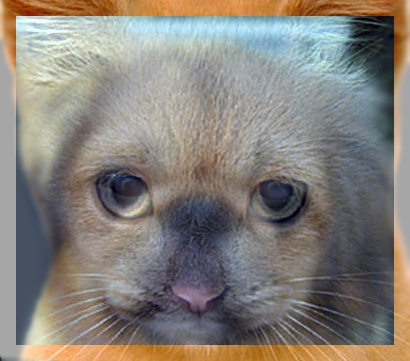
\includegraphics[width=0.25\textwidth]{../no_crop}
    \caption{Template convolution without cropping.}
    \label{fig:no-crop}
\end{figure}

This is not present in Fourier however, because the kernel is padded to the same size of the image.

\subsection{Fourier Method}
The Fourier convolution gives an equivalent to template convolution, except is more computationally efficient by working instead in the frequency domain.

\inputminted[
    firstline = 64,
    lastline = 88
]{python}{../hybrid.py}

\subsection{Speed Comparison}
The speed difference between the ``brute-force'' and Fourier methods is noticeable when you run the script. The official time comparisons are given below:

\begin{minted}[
    frame=single,
    fontsize=\footnotesize,
    tabsize=4
]{text}
time ./hybrid.py -i data/dog.bmp data/cat.bmp -c 4 4 -o hybrid.jpg -v visual.jpg  
    6.68s user 0.15s system 80% cpu 8.496 total
    
time ./hybrid.py -i data/dog.bmp data/cat.bmp -c 4 4 -o hybrid.jpg -v visual.jpg -f 
    0.67s user 0.13s system 156% cpu 0.510 total
\end{minted}

\section{Gaussian Filters}
To low pass filter an image, convolve the Gaussian filter -- of particular cutoff frequency, $\sigma$ -- with the original image. One can simply subtract the low pass filtered result from the original image in order to produce the high pass filter equivalent.

\inputminted[
    firstline = 103,
    lastline = 126
]{python}{../hybrid.py}

\begin{figure}[!htbp]
    \centering
    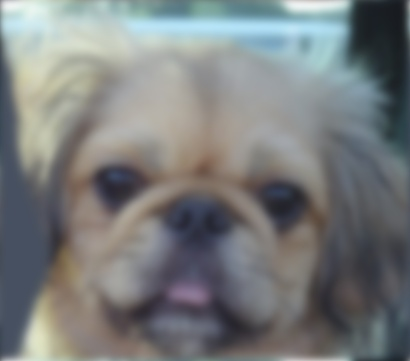
\includegraphics[width=0.25\textwidth]{../low}
    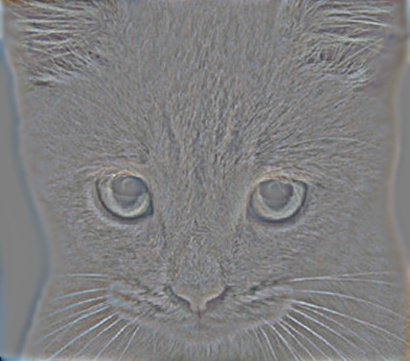
\includegraphics[width=0.25\textwidth]{../high}
    \caption{Low and high pass filtered images with $\sigma=4$.}
    \label{fig:high-low}
\end{figure}

Notice in figure~\ref{fig:high-low} the boarder around the images. This is padding due to the iterative convolution method, and would not otherwise be present in the equivalent operation using the Fourier method.

\section{Hybrid Images}
Hybrid images are formed by summing together a low-pass filtered image, with a high-pass filtered, but different, image. The higher frequencies dominate when the viewing distance is short, however the lower frequencies dominate at a larger distance. The effect of hybrid images is shown in figure~\ref{fig:visual}.

\begin{figure}[!htbp]
    \centering
    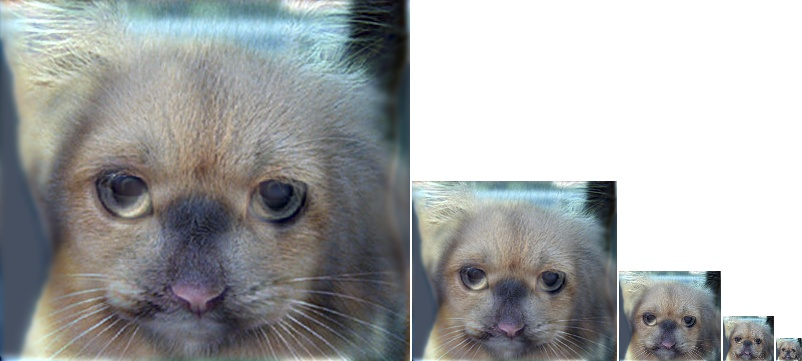
\includegraphics[width=0.5\textwidth]{../visual}
    \caption{Visualising the effect of hybrid images filtered with $\sigma=4$.}
    \label{fig:visual}
\end{figure}

\section{Usage}
The \texttt{argparse} python module was used to generate arguments for the script. It allows the user to define kernel sizes -- for applying arbitrary sized Sobel templates for example -- low/high cutoff frequencies for the Gaussian filter, input images to process and output destinations for the hybrid result and the visualisation.

\begin{minted}[
    frame=single,
    fontsize=\footnotesize,
    tabsize=4
]{text}
usage: hybrid.py [-h] -i IMAGE IMAGE [-k KERNEL KERNEL] [-c CUTOFF CUTOFF]
                 [-o OUTPUT] [-v VISUAL] [-f] [-s]

optional arguments:
  -h, --help            show this help message and exit
  -i IMAGE IMAGE, --image IMAGE IMAGE
                        Path to input images.
  -k KERNEL KERNEL, --kernel KERNEL KERNEL
                        Kernal size, e.g. 5 7. Note: first image in list will
                        be used.
  -c CUTOFF CUTOFF, --cutoff CUTOFF CUTOFF
                        Gaussian cutoff frequencies, e.g. 5 5.
  -o OUTPUT, --output OUTPUT
                        Path to output image file.
  -v VISUAL, --visual VISUAL
                        Path to output visualisation file.
  -f, --fourier         Use Fourier convolution.
  -s, --sobel           Run Sobel edge detection on the first image.
\end{minted}

Example usage is shown below, with the convolution taking place between ``dog.bmp'' and ``cat.bmp'' with the cutoff frequency of $\sigma=4$ for both low and high pass. The output hybrid image is saved to ``hybrid.jpg'' and the visualisation is saved to ``visual.jpg''. The final flag indicates that the Fourier method of convolution will be used.
\begin{minted}[
    frame=single,
    fontsize=\footnotesize,
    tabsize=4
]{text}
> ./hybrid.py -i data/dog.bmp data/cat.bmp -c 4 4 -o hybrid.jpg -v visual.jpg -f
[data/dog.bmp]	Generating low pass image...
[data/dog.bmp]	Calculating Gaussian kernel...
[data/cat.bmp]	Generating high pass image...
[data/cat.bmp]	Calculating Gaussian kernel...
Creating hybrid image...
Creating visualisation...
Done.
\end{minted}

\section{Other Kernels}
To demonstrate the convolution further, the script offers support for additional kernels. You will note that these other convolutions only act on the first image entered with the \texttt{-i} flag. This is to reduce script complexity yet demonstrating the working concept.

\subsection{Sobel Edge Detection}
Sobel edge detection applies the 2-dimensional kernels shown in the code below. 

\inputminted[
    firstline = 225,
    lastline = 231
]{python}{../hybrid.py}

This kernel can be applied to the first image in the two element list using the \texttt{-s} flag, as shown below.

\begin{minted}[
    frame=single,
    fontsize=\footnotesize,
    tabsize=4
]{text}
> ./hybrid.py -s -i Data/bicycle.bmp Data/motorcycle.bmp
\end{minted}

\begin{figure}[!htbp]
    \centering
    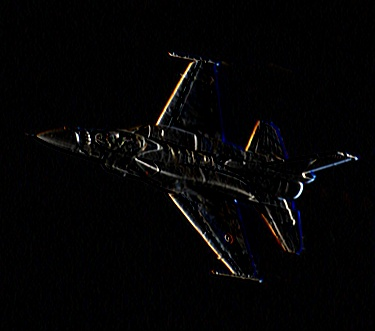
\includegraphics[width=0.25\textwidth]{../sobel_x}
    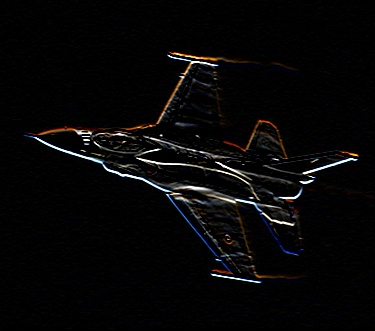
\includegraphics[width=0.25\textwidth]{../sobel_y}
    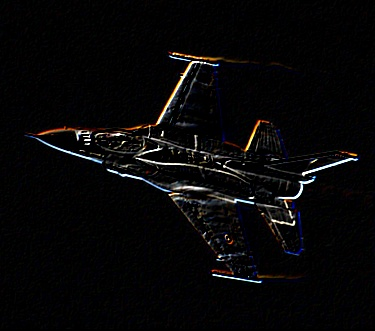
\includegraphics[width=0.25\textwidth]{../sobel_xy}    
    \caption{Sobel edge detection applied in the horizontal, vertical and combined plane.}
    \label{fig:high-low}
\end{figure}

\subsection{Arbitrary Blur}
The \texttt{-k} flag allows you to set the size of a simple blurring kernel. The kernel is simply an array of ones, divided by the product of the dimensions specified -- with a 255 scaling for increased display visibility. 

\inputminted[
    firstline = 207,
    lastline = 207
]{python}{../hybrid.py}

Within the \texttt{main} function, the template convolution is used for arbitrary kernels to help demonstrate the effect of asymmetric dimensions on the image border. This can be seen in the border of figure~\ref{fig:arb-kern}

\begin{minted}[
    frame=single,
    fontsize=\footnotesize,
    tabsize=4
]{text}
> ./hybrid.py -k 15 3 -i Data/cat.bmp Data/dog.bmp -o arb.jpg
\end{minted}

\begin{figure}[!htbp]
    \centering
    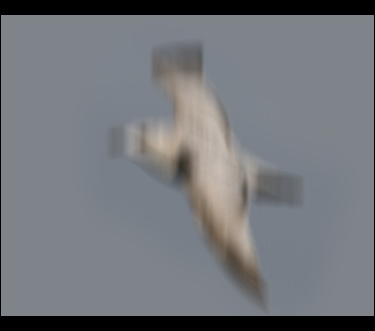
\includegraphics[width=0.25\textwidth]{../arb}
    \caption{Simple blur with a kernel size of $15\times 3$.}
    \label{fig:arb-kern}
\end{figure}

\end{document}